% *********************************************************************
% © 2021–2024 Jeremy Sylvestre
%
% Permission is granted to copy, distribute and/or modify this document
% under the terms of the GNU Free Documentation License, Version 1.3 or
% any later version published by the Free Software Foundation; with no
% Invariant Sections, no Front-Cover Texts, and no Back-Cover Texts. A
% copy of the license is included in the appendix entitled “GNU Free
% Documentation License” that appears in the output document of this
% PreTeXt source code. All trademarks™ are the registered® marks of
% their respective owners.
%
% *********************************************************************

\newcommand*{\xmin}{0}
\newcommand*{\xmax}{3}
\newcommand*{\ymin}{-3}
\newcommand*{\ymax}{4}

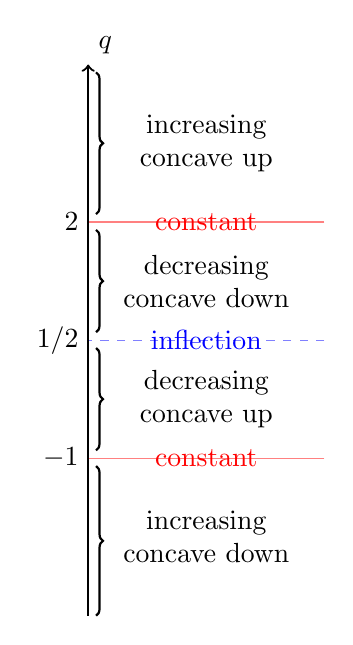
\begin{tikzpicture}
[
	closedpt/.style={circle,draw,fill,inner sep=0pt,minimum size=4pt},
	openpt/.style={circle,draw,inner sep=0pt,minimum size=4pt}
]

	\foreach \q in {-1,2} {
		\draw[red!50!white] (\xmax,\q) -- (\xmin,\q);
		\node[left] at (0,\q) {$\q$};
		\node[red] at (1.5,\q) {constant};
	}

	\draw[dashed,blue!50!white] (\xmax,0.5) -- (\xmin,0.5);
	\node[left] at (0,0.5) {$1/2$};
	\node[blue] at (1.5,0.5) {inflection};

	\draw[thick, decorate, decoration = {brace}, xshift=0.1cm] (0,-1.1) -- (0,\ymin);
	\node[align=center] at (1.5,-2) {increasing \\ concave down};

	\draw[thick, decorate, decoration = {brace}, xshift=0.1cm] (0,0.4) -- (0,-0.9);
	\node[align=center] at (1.5,-0.25) {decreasing \\ concave up};

	\draw[thick, decorate, decoration = {brace}, xshift=0.1cm] (0,1.9) -- (0,0.6);
	\node[align=center] at (1.5,1.25) {decreasing \\ concave down};

	\draw[thick, decorate, decoration = {brace}, xshift=0.1cm] (0,3.9) -- (0,2.1);
	\node[align=center] at (1.5,3) {increasing \\ concave up};

	% axes
	% \draw[->,thick] (\xmin,0) -- (\xmax,0) node[below right] {$x$};
	\draw[->,thick] (0,\ymin) -- (0,\ymax) node[above right] {$q$};

\end{tikzpicture}
